\subsection{Introduction}
%LET'S GO TEAM!!! ONE LESS SECTION
%We are unstoppppable --> DAB DAB DAB

To design Astrea constellation the orbit parameters must be decided following the stablished requirments. As seen in the previous sections, there are different types of constellation that must be considered when selecting those parametrs. 

The main requirement in the bases of this chapter is to fulfill global coverage of the Earth. Therefore all the possibles solutions have to be tested to ensure they pass this specification.


\subsection{Method Bases}

The testing method is deigned to evaluate the achievment of global coverage. The main variables needed for the development of it are the following:

\begin{table}[H]
\centering
\begin{tabular}{|c|l|}
\hline
\multicolumn{2}{|c|}{Coverage Testing Method Variables}     \\ \hline
$$typeC$$          & Type of constellation        			 \\ \hline
$\varepsilon$      & Elevation angle {[}º{]}                  \\ \hline
$$h$$              & Height  {[}km{]}                          \\ \hline
$$in$$             & Inclination angle {[}º{]}                 \\ \hline
$n_{p}$            & Number of Planes                          \\ \hline
$N_{pp}$           & Number of Satellites per plane            \\ \hline
\end{tabular}
\caption{Coverage Testing Method main Variables}
\end{table}  

It consist in evaluating all the possible variables combinations within established margins and  testing them to know if they fulfill the determined conditions than ensures global coverage.
%Figure~\ref{fig:AngleSSatFoot} shows the complete algorithm for this method.\\

\subsubsection{Global Coverage Conditions}


\textbf{Same plane condition}\

In order to fulfill the desired coverage, the distance between two satellites on the same plane must not be more than two times the central angle $\beta$. This condition is visually represented in Figure~\ref{fig:ConditionGCoverage} .\\

\textbf{Different plane condition}\

To accomplish the coverage requirments, the distance between two satellites on different planes must not be more than the central anglep $\beta$. This condition is visually represented in Figure~\ref{fig:ConditionGCoverage} .\\

\begin{figure}%[H] %[b] % h / H / b / t
	\centering
	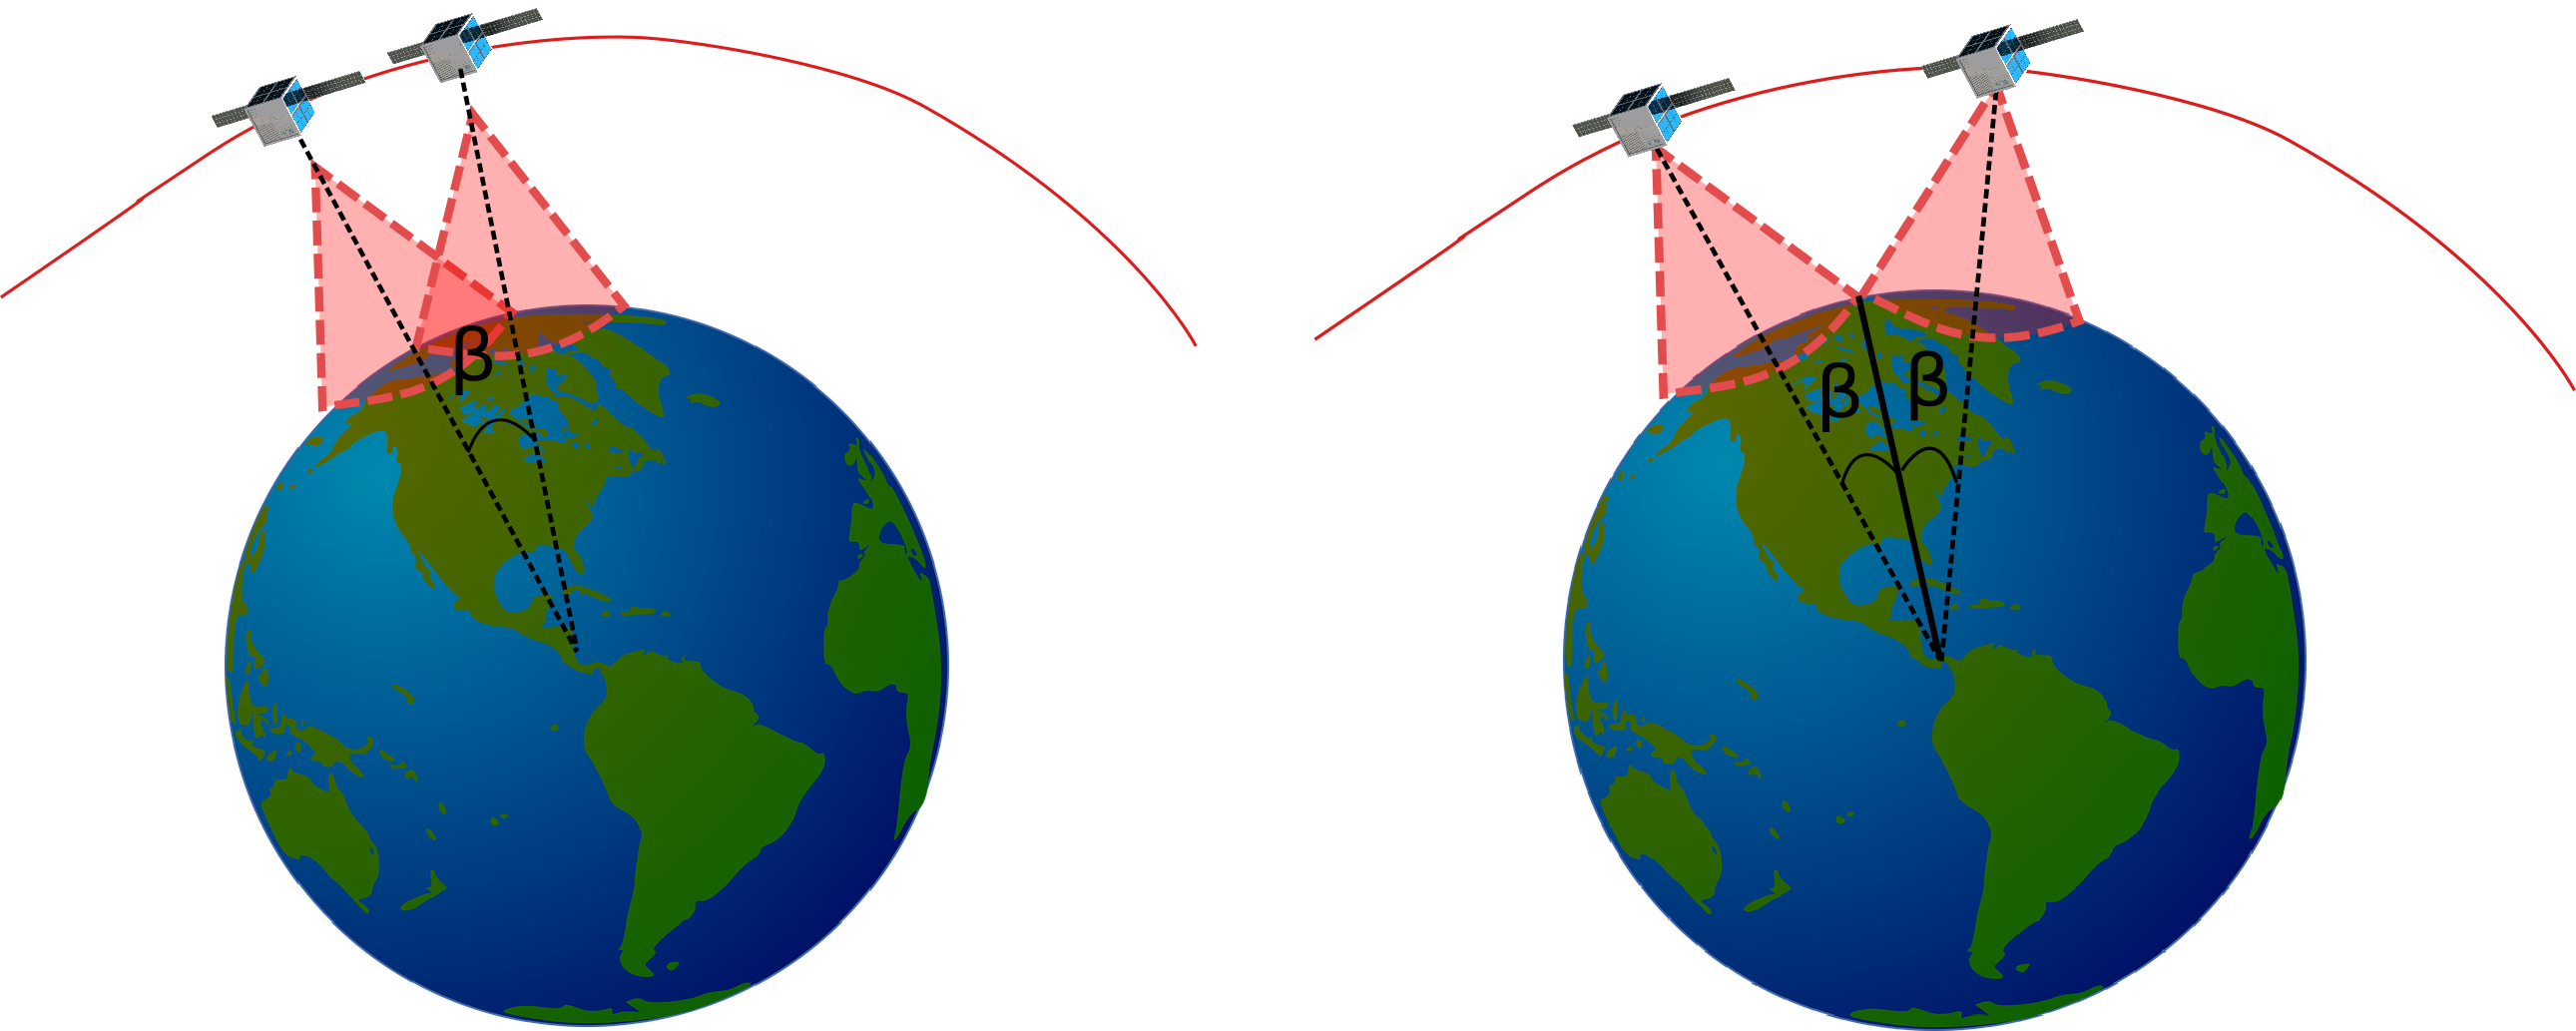
\includegraphics[width=.8\textwidth]{./testing/ConditionGCoverage.png}\\
	\caption{Geometrical conditions needed to fulfill global coverage.\\
			On the left: Condition between satellites of different planes.\\
			On the right: Condition between satellites of the same plane}
	\label{fig:ConditionGCoverage}
\end{figure}

\subsubsection{Results of Testing Method}

A MATLAB routine has been designed to compute the describe algorithm. In this phase different values of all the variables have been computed in order to found the most suitable solution. The values tested are the following:


\begin{table}[H]
\centering
\begin{tabular}{|c|l|}
\hline
\multicolumn{2}{|c|}{Coverage Testing Method Variables}     \\ \hline
$$typeC$$          & {[}180 210 225 240 360{]} {[}º{]} 			 \\ \hline
$\varepsilon$      & {[}20{]} {[}º{]}                         \\ \hline
$$h$$              & {[}540-550{]} {[}km{]}                   \\ \hline
$$in$$             & {[}70-80{]} {[}º{]}                 \\ \hline
$n_{p}$            & {[}5-12{]}                        \\ \hline
$N_{pp}$           & {[}10-24{]}                    \\ \hline
\end{tabular}
\caption{Testing Values for the Coverage Testing Method}
\end{table}  

\textbf{General Solution}\\

The program has been runned for all the range specified above to see the evolution of a satellite network configuration regarding the variation of the orbital parameters in order to find the best constellations options.

As it can be deduced both the number of planes and satellites decreases when increasing height because as explained before the footprint of the satellites gets incremented with height.
If height is left as a constant, a less intuitive results are obtain. We have now different configurations in terms of number of satellites an planes due to the variation of the inclination angle of the planes.
In the Figure~\ref{fig:graph120} is shown the results obtained for one of the analysed configurations. \\

\begin{figure}%[H] %[b] % h / H / b / t
	\centering
	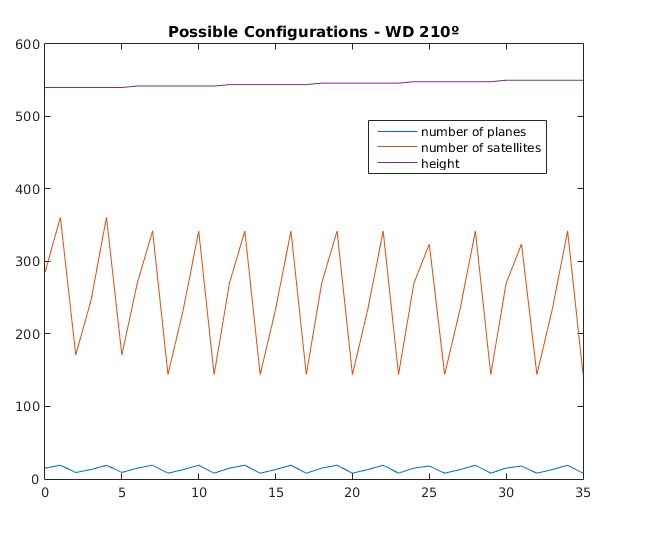
\includegraphics[width=.6\textwidth]{./testing/graph210.png}\\
	\caption{Possible satellite configurations for a 210º Walker Delta configuration}
	\label{fig:graph120}
\end{figure}

Once all the possible configurations have been computed, the ground track of three of them  has been ploted to visualy check the coverage obtained. 

\begin{figure}%[H] %[b] % h / H / b / t
	\centering
	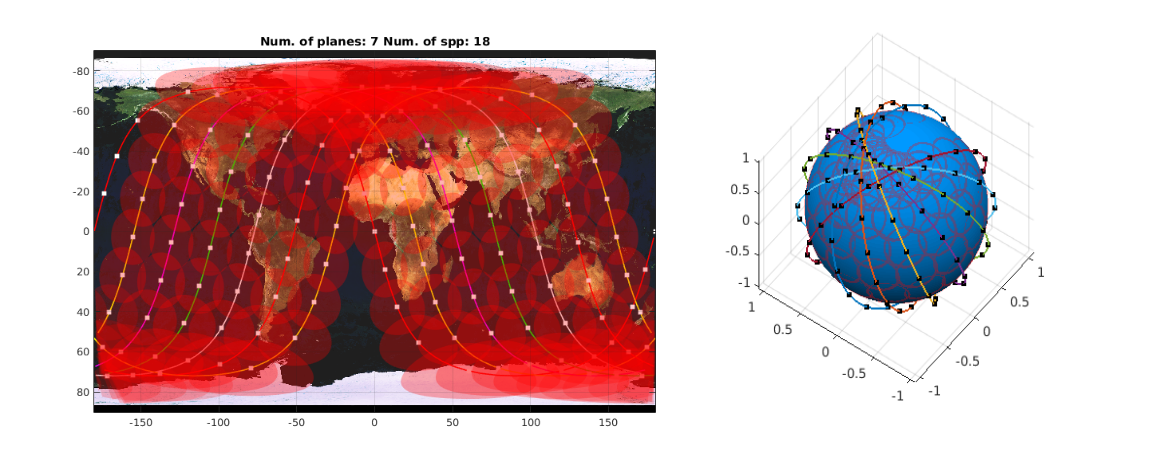
\includegraphics[width=1\textwidth]{./testing/WB180.png}\\
	\caption{Ground track and spherical representation for a 180º Walker Delta configuration}
	\label{fig:graph120}
\end{figure}

\begin{figure}%[H] %[b] % h / H / b / t
	\centering
	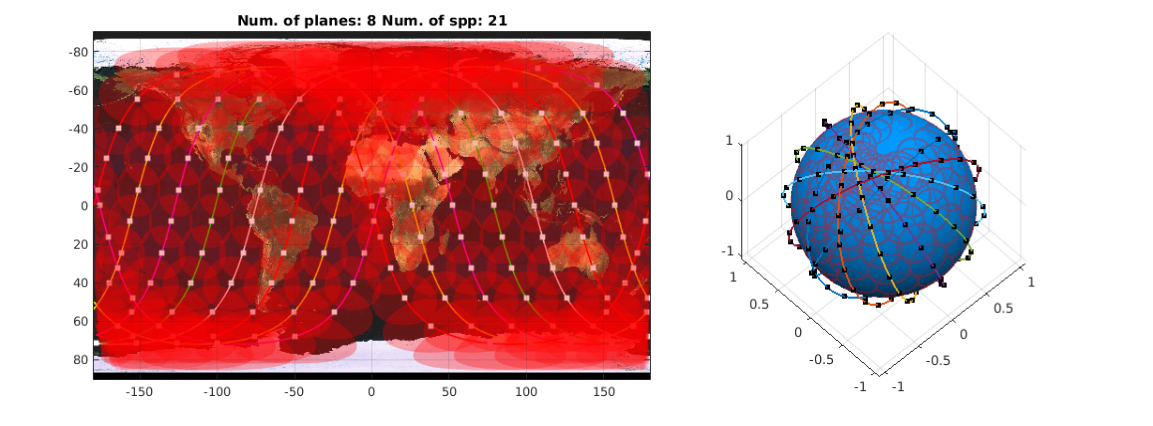
\includegraphics[width=1\textwidth]{./testing/WB210.png}\\
	\caption{Ground track and spherical representation for a 210º Walker Delta configuration}
	\label{fig:graph120}
\end{figure}

\begin{figure}%[H] %[b] % h / H / b / t
	\centering
	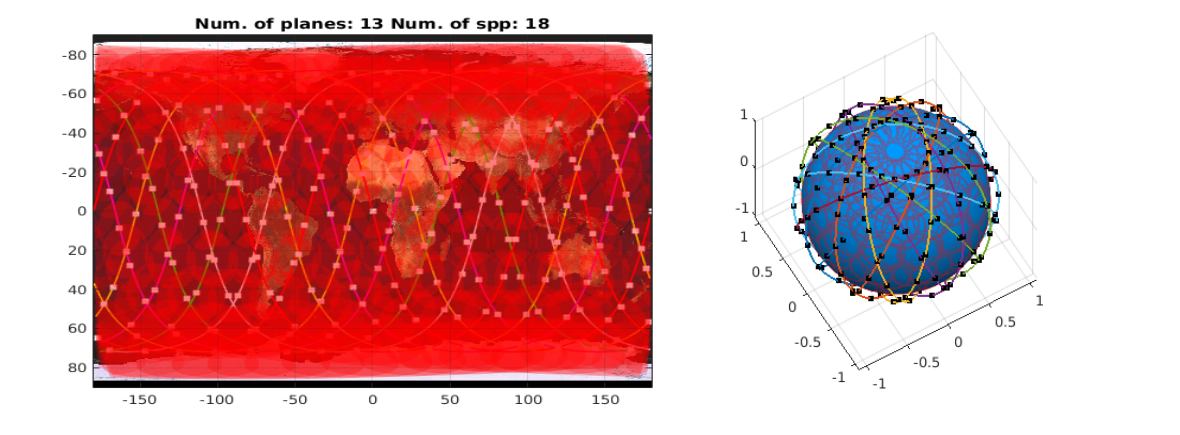
\includegraphics[width=1\textwidth]{./testing/WB360.png}\\
	\caption{Ground track and spherical representation for a 360º Walker Delta configuration}
	\label{fig:graph120}
\end{figure}

 
\textbf{Conclusions}\\  
From the developed code that runs all the parameters needed to define a Walker Delta configuration it is possible to obtain for a chosen requirment which are the optimum configuration. Therefore defining the criteria in function of the constellation needs it will be possible to optimize the design. 
The configurations that will be later considered to perform an analysis of weighted weights are extracted from this routine.